\chapter{Using File Systems}\label{ch:04-file-use}

\section{Tree Structure}

The information in a file system is organised in a tree.
Here is a (partial) tree of a UNIX-like operating system:
  \tikzset{c/.style={inner sep=2pt,circle,fill}}
  \tikzset{e/.style={sloped,above}}
\begin{center}\small
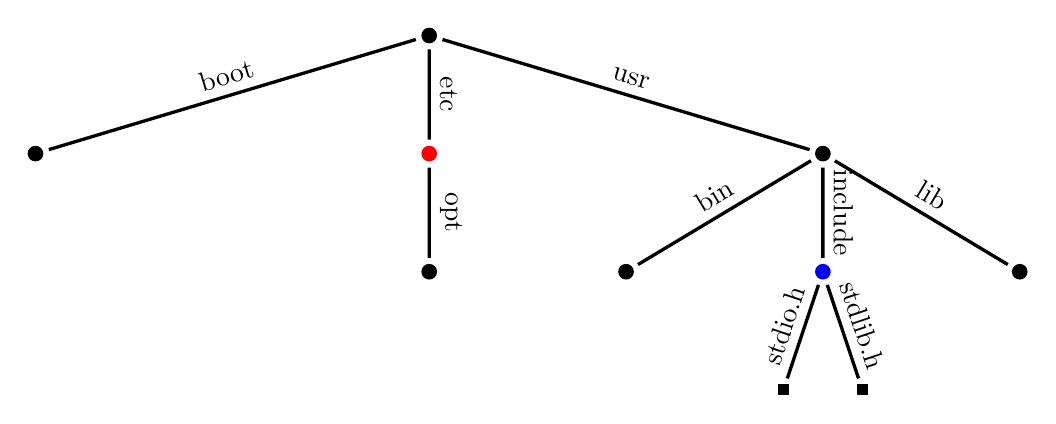
\begin{tikzpicture}
  [level distance=15mm,
  edge from parent/.style={very thick,shorten >=2pt,shorten <=2pt,draw},
  every child node/.style={c},
  level 1/.style={sibling distance=50mm},
  level 2/.style={sibling distance=25mm},
  level 3/.style={sibling distance=10mm}]
  \node[c] {}
    child { node{}
      edge from parent node[e] {boot}
    }
    child { node[fill=red]{}
      child { node{}
        edge from parent node[e] {opt}
      }
      edge from parent node[e] {etc}
    }
    child { node{}
      child { node{}
        edge from parent node[e] {bin}
      }
      child { node[fill=blue]{}
        child { node[rectangle]{}
          edge from parent node[e] {stdio.h}
        }
        child { node[rectangle]{}
          edge from parent node[e] {stdlib.h}
        }
        edge from parent node[e] {include}
      }
      child { node{}
        edge from parent node[e] {lib}
      }
      edge from parent node[e] {usr}
    }
  ;
\end{tikzpicture}
\end{center}
We can describe the path
  from~\tikz{\node[c,fill=red]{};} to~\tikz{\node[c,fill=blue]{};}
  by~`\.{../usr/include}'.
The path
  from~\tikz{\node[c,fill=blue]{};} to~\tikz{\node[c,fill=red]{};}
  could be described
  by~`\.{../../etc/opt/..}'.
The path's steps are separated by slash~\.{/}.
A step either goes up (\.{..}) or goes down along the named edge.
(We can only go up from a \tikz{\node[c]{};}:
  If a path reaches a~\tikz{\node[c,rectangle]{};}, then it's stuck there.)
Such paths are called \df{relative paths},
  and their starting point is the \df{current working directory} of the process.
\df{Absolute paths} use the root of the tree as their starting point,
  rather than the current working directory.
Absolute paths are described by similar strings,
  except the strings start with a slash.
For example,
  both \.{/etc} and \.{/etc/opt/..} are absolute paths
  to~\tikz{\node[c,fill=red]{};}.

The circles~\tikz{\node[c]{};} represent \df{directories},
  which are files that have children.
The downward pointing edges represent \df{directory entries}.
The squares~\tikz{\node[c,rectangle]{};} represent non-directory files,
  which are leaves of the tree.
Normal files support read and write operations.

\smallskip

On POSIX operating systems there is only one file system tree.
If you know that one computer may have both a hard drive and a DVD,
  then you may wonder how come there could be only one tree.
To answer this, take a look in the \.{/dev} directory:
\begin{verbatim}
rg@rg-2016:notes$ ls /dev/sda*
/dev/sda  /dev/sda1  /dev/sda2  /dev/sda3  /dev/sda4  /dev/sda5  /dev/sda6  /dev/sda7
\end{verbatim}
The file \.{/dev/sda} contains all the content of a hard drive.
The other ones are different partitions on the same hard drive.
But, how do we see the files in one of those partitions?
We \df{mount} that file:
\begin{verbatim}
mount /dev/sda1 /some/dir
\end{verbatim}
The \.{/some/dir} must exist prior to running the command.
After the command is run, \.{/some/dir}
  will contain the files on the partition \.{/dev/sda1}.

So, what's going on here?
The operating system shows us a \df{VFS (virtual file system)}.
Files appear and disappear in the directory \.{/dev}
  depending on which hardware devices the operating system detects.
The operating system gives us access to a wide range of devices using
  a uniform interface for interacting with files.
We can tell the operating system, as we did above,
  that some of these devices contain real file systems,
  and thus grow subtrees in the unique VFS tree.


\section{Security}

POSIX operating systems support at least the following basic system of permissions.
Suppose we list details about a file:
\begin{verbatim}
rg@rg-2016:notes$ ls -l 03-file-use.tex
-rw-rw-r-- 1 rg rg 3538 Mar 18 17:35 03-file-use.tex
\end{verbatim}
The first column contains three sets of permissions, namely
  (1)~the user permissions \hbox{\.{r\,w\,-}},
  (2)~the group permissions \hbox{\.{r\,w\,-}}, and
  (3)~the other permissions \hbox{\.{r\,-\,-}}.
Each of those is a subset of \.{rwx}:
  \.{r} means `allowed to read',
  \.{w} means `allowed to write',
  \.{x} means `allowed to execute'.
Given a set of permissions, it is pretty clear what we are allowed to do.
But, there are \emph{three} sets.
Which one are we supposed to use?
This is determined as follows.
Each file has an owner and a group:
  these are listed in the columns 3~and~4 above, and both are \.{rg}.
Each user belongs to a set of groups; for example:
\begin{verbatim}
rg@rg-2016:notes$ groups
rg adm cdrom sudo dip plugdev lpadmin sambashare
\end{verbatim}
If the owner of a file tries to access it,
  then the set~(1) of permissions is used.
Otherwise, if the user accessing the file belongs to the group of the file,
  then the set~(2) of permissions is used.
Otherwise, the set~(3) of permissions is used.

\smallskip

Apart from permissions, one could also use encrypted file systems.


\section{Reading and Writing Files}

POSIX defines two interfaces for interacting with files,
  a high-level one and a low-level one.
Here is an example of using the high-level interface:
\begin{ccode}
#include <stdio.h>
int main() {
  printf("Hello world!\n");
}
\end{ccode}
And here is an example of using the low-level interface:
\begin{ccode}
#include <unistd.h>
int main() {
  write(STDOUT_FILENO, "Hello world!\n", 13);
}
\end{ccode}
The high-level interface prints a string to the terminal.
The low-level interface makes it clear that printing a string
  is actually done by writing to a special file,
  following the `everything is a file' philosophy of POSIX\null.
The low-level interface also makes it clear that we want to write $13$~bytes.
Apart from forcing us to specify some uninteresting details,
  the low-level has yet another quirk:
  there is no guarantee that the string is actually printed.
If we want to make sure that `Hello world!' is printed then we have to use a loop:
\begin{ccode}
#include <unistd.h>
int main() {
  const char * buf = "Hello world!\n";
  int written = 0;
  while (written < 13) {
    written += write(STDOUT_FILENO, buf + written, 13 - written);
  }
}
\end{ccode}
Why would \.{write} return before it writes $13$~bytes?
One possible reason is that the call is interrupted by a signal.

In both the high-level and the low-level interface,
  one interacts with files in three phases:
\begin{enumerate}
\item open the file to obtain a \emph{file handle}
\item read from the file, write to the file, repeatedly
\item close the file
\end{enumerate}
For the high-level interface, the file handle is called a \df{stream},
  and it is a pointer to a \.{FILE} structure.
For the low-level interface, the file handle is called a \df{descriptor},
  and it is a nonnegative \.{int}.
Thus, the high-level interface is sometimes called the stream-based interface,
  while the low-level interface is sometimes called the descriptor-based interface.

Let us implement a program that copies a file,
  using the descriptor-based interface.
We open and close the files as follows:
\begin{ccode}
  int in_file = open(argv[1], O_RDONLY);
  int out_file = open(argv[2], O_WRONLY|O_CREAT|O_TRUNC, 0664);
  // TO BE FILLED
  close(in_file);
  close(out_file);
\end{ccode}
The function \.{open} takes a path, which can be absolute or relative,
  and returns a file descriptor.
Above, we assume that the path of the source is in \.{argv[1]}
  and the path of the target is in \.{argv[2]}.
The function \.{open} takes a second argument
  which specifies how the file should be opened.
\.{O\_RDONLY} means we will only read;
  \.{O\_WRONLY} means we will only write;
  \.{O\_CREAT} means that the file should be created if it does not exist;
  \.{O\_TRUNC} means that the content of the file should be truncated (erased).
The second argument is a bitmask,
  so we can combine flags with the bitwise logical-or operator.
Optionally, the function \.{open} takes a third argument.
The third argument says which permissions should be used in case
  the file is created.
Recall that we need three sets of permissions,
  each set being specified by three bits.
The literal \.{0664} is an \emph{octal} number, because it starts with~\.{0}.
(This is a lexical convention used by C and by many other languages.)
Each octal digit corresponds to $\ldots$ three bits.
So, each digit specifies one set of permissions:
  \.{0664} stands for {\tt rw-rw-r--}.

After opening and before closing the files,
  we do the actual copying:
\begin{ccode}
  const int buffer_size = 1 << 20; // 1 MiB
  char buffer[buffer_size];
  while (1) {
    ssize_t r = read(in_file, buffer, buffer_size);
    if (r == 0) break;
    ssize_t w = 0;
    while (w < r) w += write(out_file, buffer + w, r - w);
  }
\end{ccode}
You can find the full code in the file \.{copy.c}.

We can copy files using four functions:
\begin{ccode}
int open(const char *pathname, int flags);
int open(const char *pathname, int flags, mode_t mode);
int close(int fd);
ssize_t read(int fd, void *buf, size_t count);
ssize_t write(int fd, const void *buf, size_t count);
\end{ccode}
The function \.{open} gives us a file descriptor,
  provided a pathname in the VFS\null.
The function \.{close} closes a file descriptor.
The functions \.{read} and \.{write} let us transport data to and from the file.


\section{Synchronous I/O Multiplexing}

Suppose a process needs to read several files in parallel.
It could be that several files are ready to be read while others are not.
This would happen, for example,
  if we would implement a server and the files were network connections.
If the process calls \.{read} to get data from a file that has no data ready,
  then the process's execution would be blocked until some data becomes available.
In the meantime,
  the other files, which may have data ready, are ignored.
How should we handle such a situation?
One solution is to have multiple threads, each thread reading from one file only ---
  this is \df{asynchronous I/O multiplexing}.
Another solution is to first ask which files have data ready ---
  this is \df{synchronous I/O multiplexing}.

Let us see how synchronous I/O multiplexing works on an example.
We shall avoid using the network for now.
Instead, we use a special kind of file called `fifo file' or `named pipe'.
Let's create two of these:
\begin{verbatim}
rg@rg-2016:files$ mkfifo one two
rg@rg-2016:files$ ls -l one two
prw-rw-r-- 1 rg rg 0 Mar 19 17:16 one
prw-rw-r-- 1 rg rg 0 Mar 19 17:16 two
\end{verbatim}
We will put data into these files using the cat command.
In one terminal we run \.{cat - $>$ one},
  in another terminal we run \.{cat - $>$ two}.
We'd like a to write program that is run by
\begin{verbatim}
rg@rg-2016:files$ ./counter one two
\end{verbatim}
and periodically prints how many bytes came through \.{one} and \.{two} together,
  \emph{no matter in which order we type in the two terminals}.
You can see a complete solution in the accompanying \.{counter.c}.
Here, let us look at its main bits.

The main loop looks as follows:
\begin{ccode}
while (1) {
  // <Setup nfds and all>
  select(nfds, &all, 0, 0, 0);
  // <Read from all files in all>
}
\end{ccode}
The variable \.{all} is a set of file descriptors from which we wish to read.
The function \.{select} returns when there exists some subset of file descriptors
  on which we can call \.{read} without a blocking fear.
Moreover, \.{select} modifies the set \.{all},
  so that it now contains only those files on which it's safe to call \.{read}.

Before entering the loop from above,
  we first open all files of interest.
\begin{ccode}
int files[n];
for (int i = 0; i < n; ++i) files[i] = open(argv[i+1],O_RDONLY);
\end{ccode}
At the beginning of each iteration of the main loop,
  we set up \.{all} by inserting into it all file descriptors we still have.
We will make sure that each element of \.{files} is either a file descriptor
  of an open file, or it is~$-1$.
\begin{ccode}
fd_set all;
FD_ZERO(&all);
for (int i = 0; i < n; ++i) if (files[i] != -1) FD_SET(files[i], &all);
\end{ccode}
(We also need to set \.{ndfs} to $1+\max\.{all}$. That's easy.
  See \.{counter.c} if you don't think so.)

After the call to \.{select},
  we look at each file descriptor still in \.{all},
  and we process it.
Normally, we just read from it and count the bytes.
But, it could also be we reached the end of file,
  in which case we close the file.
\begin{ccode}
for (int i = 0; i < n; ++i) if (FD_ISSET(files[i], &all)) {
  ssize_t r = read(files[i], buffer, buffer_size);
  if (r == 0) { // end of file reached
    close(files[i]);
    files[i] = -1;
  }
  total += r;
  // <Report total>
}
\end{ccode}

The stream-based interface does not support synchronous I/O multiplexing.


\section{Distributed File Systems}

% plan
%   - overview: >1 computer, gfs&hdfs, databases on top
%   - gfs assumptions
%   - gfs api
%   - gfs performance

File systems that implement the POSIX interface usually reside in one computer.
But, one computer is insufficient to store and process big data.
A \emph{distributed file system} is similar to a normal file system,
  but with two important differences:
(1)~the interface is visible to many computers; and
(2)~the data is stored on many computers.
The two sets of computers, those that use the data and those that store the data,
  may or may not intersect.
The number of computers storing data is easily in the hundreds,
  more often in the thousands, and sometimes more.
Since one cheap hard disk can easily store a terabyte,
  a distributed file system has a capacity on the order of petabytes.
The ability to store and easily share so much data comes with some costs:
(1)~file system operations like reading and writing are significantly slower, and
(2)~the interface is poorer and offers fewer guarantees,
  compared to POSIX\null.
It should be noted that even
  the POSIX file system interface is too low level for many applications.
Instead, most applications use databases, such as MySQL,
  which are built on top of file systems.
Since distributed file systems have interfaces that are even more low-level,
  the need for database systems built on top is more acute.

Two examples of distributed file systems are
  GFS (Google File System)
  and HDFS (Hadoop File System).
The new version of GFS is called Colossus,
  but not much about it is public;
  on top of Colossus, Google has a distributed database called Spanner~[4].
Facebook, on the other hand,
  built directly a distributed database, called Cassandra~[5],
    without basing it on a distributed file system.

\smallskip

Let us now look at the design of GFS~[3].
Almost all files in GFS have at least $100$~MiB\null.
The reason for this is easy to see:
  smaller files can easily be stored and processed by a single computer,
  so it is more convenient to store them in a local file system.
For GFS files, the common use case is the following.
Several computers concurrently and regularly write to the file,
  and every once in a while a computer reads the file from start to end.
Moreover,
  these computers that use data care more about bandwidth than about latency.

\smallskip

The interface offered by GFS to client programs contains several operations
  that are familiar from POSIX:
  \.{create}, \.{delete}, \.{open}, \.{close}, \.{read}, \.{write}.
There are also two new operations:
  \.{snapshot} and \.{record append}.
To speed up the common use case,
  GFS optimises for reading sequentially from files and for appending records.
The other operations, such as writing in the middle of an existing file,
  are supported but are significantly slower.
What is the difference between writing at the end of the file,
  and appending a record?
Appending is guaranteed to be atomic.
To understand what atomic means,
  it is best to start first by understanding what non-atomic means.
Suppose two different computers try to write to the same are of a file.
This area may or may not be at the end of the file.
But, in any case, the question is what should the result be?
GFS only promises that the result will some mixture of the two writes,
  but makes no guarantees
    about which bytes come from one write operation
    and which bytes come from the other write operation.
This is non-atomic behaviour.
The reason for non-atomic behaviours, in general, is performance:
  the system (GFS in our case) would be too slow otherwise.
We will see how the implementation of GFS leads to non-atomic behaviour,
  in the next lecture.

To achieve atomicity, there are two basic implementation strategy:
  pessimistic and optimistic.
The pessimistic strategy is to serialise write operations,
  using some mutual exclusion mechanism.
In this strategy, there would be some extra communication between computers,
  whose purpose would be to ensure that write operations happen one after another.
On the other hand,
  the optimistic strategy is not to ensure mutual exclusion
    but to detect if a concurrent write operation happened.
If it did, then retry.
The \emph{record append} operation uses the second, optimistic strategy.
The computer that uses GFS is not aware of this mechanism.
All that is visible is that the record is eventually written,
  and that its bytes are not mingled with those of another write or append operation.

The \emph{snapshot} operation allows one to quickly make a copy of file,
  using a copy-on-write mechanism.

\smallskip

In 2003, when GFS was made public,
  one of its largest instances had $>300$~TiB of space,
  the average read rate was $\sim400$~MiB/s,
  and the average write rate was $\sim100$~MiB/s.
These numbers are out of date, but I'm unsure if newer ones are available publicly.
For example, HDFS, which is an open source file system similar to GFS,
  is on record with instances as big as $200$~PiB,
  which is a thousand times bigger~[6].


\section{Exercises}

\begin{enumerate}
\item
  $\blacktriangleright$
  What is an absolute path of~\tikz{\node[c,fill=blue]{};}?
\item
  Read `\.{man path\_resolution}'.
\item
  The file system tree is actually a directed graph.
  Read about file system links (hard and soft).
\item
  Read `\.{man mount}'.
\item
  Which command is used to change the owner of a file?
  Which command is used to change the group of a file?
  [Hint: Google.]
\item
  Which of the \.{rwx} permissions on a directory \.{foo}
    are needed to be able to change the current directory
    to a subdirectory of \.{foo}?
  [Hint: Just try it.]
\item
  $\blacktriangleright$
  Implement a function
\begin{javacode}
  boolean hasAccess(
    char accessType,
    String user, String[] userGroups,
    String fileOwner, String fileGroup, String permissions);
\end{javacode}
  For example, the call
\begin{javacode}
  hasAccess('w', "rg", new String[]{"foo","staff"}, "frmb", "staff", "rwxr-----");
\end{javacode}
  should return \.{false}.
  You may use any language (but you'll have to adapt the function signature).
\item
  The `Hello world!' examples do not handle errors properly.
  See \.{man printf} and \.{man 2 write} for which errors could occur,
    and change the program so that such errors are gracefully reported.
  At the very least, ensure that the program does not crash in the event that
    an error occurs.
\item
  Can you think of a situation in which the return-early behaviour
    of the low-level file interface is preferable?
  [Hint: Think of \.{scanf} versus \.{read}.]
\item
  On Linux, you can see which files are open using the \.{lsof} command.
  How many files are open on your system right now?
  Run \.{man lsof}, search for `\.{TYPE}',
    to see how many types of files there are.
\item
  $\blacktriangleright$
  What is a file handle?
  What is a file descriptor?
  What is a stream?
\item
  Another interesting operation on regular files is seeking.
  Read about it by running \.{man lseek}.
\item
  Implement \.{counter.c} using asynchronous I/O multiplexing.
  What extra complication arises?
\item
  Read `\.{man select\_tut}'.
\item
  In which situation would you use synchronous I/O multiplexing?
\item
  $\blacktriangleright$
  Which GFS operations are fast and which are slow?
  Why was GFS optimised in this way?
\end{enumerate}

\section{Notes}

\begin{itemize}
\item[{[1]}]
  Linux Foundation,
  \href%
    {http://refspecs.linuxfoundation.org/FHS_3.0/fhs/index.html}%
    {Filesystem Hierarchy Standard},
  2015
\item[{[2]}]
  \href%
    {http://pubs.opengroup.org/onlinepubs/9699919799/basedefs/V1_chap04.html}%
    {General Concepts, POSIX},
  2013
\item[{[3]}]
  Ghemawat et al., \emph{The Google File System}, 2003
\item[{[4]}]
  Corbett et al., \emph{Spanner: Google's Globally Distributed Database}, 2013
\item[{[5]}]
  Lakshman, Malik, \emph{Cassandra: a decentralized structured storage system},
  2010
\item[{[6]}]
  \href{https://hortonworks.com/apache/hdfs/}%
    {\emph{Apache Hadoop HDFS}}, 2017
\end{itemize}


% vim:spell:spelllang=en_gb:
